% ============================================================
% HSBI Beamer — ISLP Lecture Series — IMPROVED EDITION
% Chapter 0b: Precourse Toolkit (notation, logs and odds, likelihood, Python)
% ============================================================
\documentclass[aspectratio=169,11pt]{beamer}
\usepackage[utf8]{inputenc}\usepackage[T1]{fontenc}\usepackage[english]{babel}
\usepackage{graphicx}\usepackage{booktabs}\usepackage{amsmath,amssymb,amsfonts}
\usepackage{mathtools}\usepackage{hyperref}\usepackage{xcolor}
\usepackage{verbatim}\usepackage{alltt}
\usepackage{tikz}\usetikzlibrary{calc,arrows.meta,positioning,shapes}
\usepackage{tcolorbox}\tcbuselibrary{skins}
\usepackage{textcomp}\providecommand{\euro}{\texteuro}

\usetheme{Madrid}\usecolortheme{default}
\setbeamertemplate{navigation symbols}{}
\setbeamertemplate{footline}[frame number]
\setbeamertemplate{blocks}[rounded][shadow=false]
\setbeamertemplate{headline}{%
  \leavevmode\hbox{%
    \begin{beamercolorbox}[wd=\paperwidth,ht=2.2ex,dp=0.9ex]{section in head/foot}%
      {\fontsize{4.6}{5.2}\selectfont%
       \insertsectionnavigationhorizontal{\paperwidth}{}{\hskip0pt plus1filll}}%
    \end{beamercolorbox}}%
}
\setbeamerfont{section in head/foot}{size=\tiny}
\setbeamerfont{palette primary}{size=\tiny}
\setbeamerfont{palette tertiary}{size=\tiny}
\setbeamerfont{section in toc}{size=\footnotesize}

\usepackage{listings}
\definecolor{pyKw}{RGB}{0,0,180}\definecolor{pyStr}{RGB}{20,120,40}
\definecolor{pyCom}{RGB}{120,120,120}\definecolor{accent}{RGB}{38,70,140}
\lstdefinestyle{Pystyle}{language=Python,basicstyle=\ttfamily\footnotesize,
  keywordstyle=\color{pyKw}\bfseries,commentstyle=\color{pyCom}\itshape,
  stringstyle=\color{pyStr},showstringspaces=false,upquote=true,
  columns=fullflexible,breaklines=true,literate={~}{{$\sim$}}1}
\lstset{style=Pystyle}

\AtBeginSection[]{\begin{frame}{Outline}\scriptsize
  \begin{columns}[t]
    \begin{column}{0.5\textwidth}
      \tableofcontents[currentsection,sectionstyle=show/shaded,
                       subsectionstyle=show/show/hide,sections={1-6}]
    \end{column}
    \begin{column}{0.5\textwidth}
      \tableofcontents[currentsection,sectionstyle=show/shaded,
                       subsectionstyle=show/show/hide,sections={7-12}]
    \end{column}
  \end{columns}
\end{frame}}

\newcommand{\islpsource}[1]{%
  \vfill\hfill{\tiny\itshape\color{gray}Source: #1 \textemdash{} ISLP, James et al.\ (2023).}\par
}

\newtcolorbox{takeaway}[1][Takeaway]{enhanced,colback=green!4,colframe=green!50!black,
  boxrule=0pt,leftrule=2.5pt,arc=2pt,fonttitle=\bfseries,title=#1,
  left=2mm,right=2mm,top=1mm,bottom=1mm}
\newtcolorbox{numexample}[1][Worked example]{enhanced,colback=orange!4,colframe=orange!70!black,
  boxrule=0pt,leftrule=2.5pt,arc=2pt,fonttitle=\bfseries,title=#1,
  left=2mm,right=2mm,top=1mm,bottom=1mm}
\newtcolorbox{readme}[1][How to read this]{enhanced,colback=blue!4,colframe=accent,
  boxrule=0pt,leftrule=2.5pt,arc=2pt,fonttitle=\bfseries,title=#1,
  left=2mm,right=2mm,top=1mm,bottom=1mm}

\title{Quantitative Research Methods}
\subtitle{Chapter 0b: Precourse Toolkit}
\author{Prof.\ Dr.\ Christoph Weisser}\institute{HSBI}
\date{Summer Semester 2026}\graphicspath{{images/}}

\newtcolorbox{exercise}[1][Exercise]{enhanced, fontupper=\footnotesize, colback=purple!4, colframe=purple!55!black, boxrule=0pt, leftrule=2.5pt, arc=2pt, fonttitle=\bfseries, title=#1, left=2mm, right=2mm, top=1mm, bottom=1mm}
\newtcolorbox{solutionbox}[1][Solution]{enhanced, fontupper=\footnotesize, colback=teal!5, colframe=teal!55!black, boxrule=0pt, leftrule=2.5pt, arc=2pt, fonttitle=\bfseries, title=#1, left=2mm, right=2mm, top=1mm, bottom=1mm}

% Reclaim ~2pt of body height (custom nav headline makes full slides tip over by ~1.83pt)
\addtobeamertemplate{frametitle}{}{\vspace{-2pt}}

\newtcolorbox{longexercise}[1][Extended exercise (15 min)]{enhanced, fontupper=\footnotesize, colback=violet!6, colframe=violet!55!black, boxrule=0pt, leftrule=3pt, arc=2pt, fonttitle=\bfseries, title=#1, left=2mm, right=2mm, top=1mm, bottom=1mm}

\newtcolorbox{labnote}[1][Run this live in the lab notebook]{enhanced, fontupper=\footnotesize, colback=cyan!7, colframe=cyan!45!black, boxrule=0pt, leftrule=3pt, arc=2pt, fonttitle=\bfseries, title=#1, left=2mm, right=2mm, top=1mm, bottom=1mm}

\begin{document}
\begin{frame}[plain]\titlepage\end{frame}

\begin{frame}{The course at a glance}
  \footnotesize
  \begin{center}
  \begin{tabular}{@{}c r l@{}}
    & \textbf{Lecture} & \textbf{Topic}\\
    \midrule
     & 0 & Precourse (a) --- statistics refresher: description, probability, inference \\
    $\blacktriangleright$ & \textbf{0b} & \textbf{Precourse (b) --- notation, logs and odds, likelihood, Python} \\
     & 1 & Ch.\ 1 + 2 --- Introduction; what is statistical learning \\
     & 2 & Ch.\ 2 --- Accuracy, bias--variance, Bayes classifier, KNN \\
     & 3--4 & Ch.\ 3 --- Linear regression (estimation, inference, diagnostics) \\
     & 5--6 & Ch.\ 4 --- Classification (logistic, LDA/QDA, naive Bayes, ROC) \\
     & 7 & Ch.\ 5 --- Resampling (validation, CV, bootstrap) \\
     & 8 & Ch.\ 6 --- Model selection and regularisation (ridge, lasso) \\
     & 9 & Ch.\ 7 --- Moving beyond linearity (splines, GAMs) \\
     & 10 & Ch.\ 8 --- Tree-based methods (trees, forests, boosting) \\
     & 11 & Ch.\ 10 --- Deep learning (MLPs, CNNs, training) \\
     & 12 & Ch.\ 13 --- Multiple testing (FWER, FDR) \\
  \end{tabular}
  \end{center}
  \vspace{2pt}
  {\scriptsize The second half of the optional precourse. Part (a) refreshed the
  \emph{statistics}; this session covers the \emph{language and machinery} the
  later chapters use without explanation.}
\end{frame}

\begin{frame}{Contents}
  \begin{columns}[t]
    \begin{column}{0.5\textwidth}
      \tableofcontents[hideallsubsections,sections={1-4}]
    \end{column}
    \begin{column}{0.5\textwidth}
      \tableofcontents[hideallsubsections,sections={5-7}]
    \end{column}
  \end{columns}
  \vfill
  {\tiny Optional and advanced material is collected in the \textbf{appendix} at the end of the deck.}
\end{frame}

\begin{frame}{Why this second session exists}
  \footnotesize
  These five topics were counted in the ten lecture decks. Each is used
  \emph{heavily} and explained \emph{nowhere} --- the chapters assume you
  already read them fluently.
  \begin{center}
  \begin{tabular}{@{}llr@{}}
    \toprule
    \textbf{Topic} & \textbf{Where it bites} & \textbf{Uses} \\
    \midrule
    $\log$ and $\exp$ & Ch.\ 4 (113), Ch.\ 10 (31), Ch.\ 6 (16) & 176 \\
    odds and the logit & Ch.\ 4 (92), Ch.\ 10 (12) & 108 \\
    likelihood and $\prod$ & Ch.\ 4 (35), Ch.\ 2--3 & 37 \\
    $\sum$, $\arg\max$, indicator, set notation & every chapter from Ch.\ 2 & 180 \\
    counting and $2^p$ cost & Ch.\ 6 (subset selection) & 13 \\
    \bottomrule
  \end{tabular}
  \end{center}
  \begin{takeaway}[The claim]
    None of this is hard. All of it is \emph{unfamiliar notation for familiar
    ideas} --- and unfamiliar notation is what makes a lecture feel
    impossible to follow.
  \end{takeaway}
\end{frame}

\begin{frame}{Notation introduced in this session}
  \footnotesize
  \begin{center}
  \begin{tabular}{@{}ll@{}}
    \toprule
    \textbf{Symbol} & \textbf{Meaning} \\
    \midrule
    $\sum_{i=1}^{n} a_i$ & add up $a_1,\dots,a_n$ \\
    $\prod_{i=1}^{n} a_i$ & multiply $a_1,\dots,a_n$ \\
    $\arg\min_\theta f(\theta)$ & the \emph{value of $\theta$} that makes $f$ smallest \\
    $I(\text{condition})$ & $1$ if the condition holds, $0$ otherwise \\
    $x \in \mathcal{S}$, $|\mathcal{S}|$ & $x$ is in the set $\mathcal{S}$; the size of $\mathcal{S}$ \\
    $\log$, $\exp$ & natural logarithm (base $e$) and its inverse $e^{x}$ \\
    $\mathrm{odds} = \frac{p}{1-p}$ & how much more likely than not \\
    $\mathrm{logit}(p) = \log\frac{p}{1-p}$ & log-odds: a probability on an unbounded scale \\
    $\sigma(z) = \frac{1}{1+e^{-z}}$ & the logistic (sigmoid) function; the inverse of the logit \\
    $L(\theta)$, $\ell(\theta)$ & likelihood and log-likelihood of the parameter $\theta$ \\
    $\hat\theta_{\mathrm{MLE}}$ & the value of $\theta$ that maximises the likelihood \\
    $\binom{p}{k}$ & the number of ways of choosing $k$ items from $p$ \\
    $2^{p}$ & the number of subsets of $p$ predictors: how the cost grows \\
    \bottomrule
  \end{tabular}
  \end{center}
\end{frame}

\begin{frame}{Learning objectives for this session}
  By the end you will be able to:
  \begin{itemize}
    \item \textbf{Read aloud} any formula in the course: sums, products,
          $\arg\max$, indicators, subscripts and set notation.
    \item \textbf{Manipulate} logs and exponentials, and explain what a
          coefficient means when the response is logged.
    \item \textbf{Convert} freely between probability, odds and log-odds, and
          explain why classification models work on the logit scale.
    \item \textbf{Write down} a likelihood, take its log, and explain what
          maximum likelihood chooses --- and why it coincides with least
          squares under normal errors.
    \item \textbf{Count} models and explain why $2^p$ makes exhaustive search
          hopeless.
    \item \textbf{Write} the Python the labs actually use: functions, loops,
          comprehensions, seeds, and the \texttt{fit}/\texttt{predict} pattern.
  \end{itemize}
\end{frame}


% ============================================================
\section{Reading mathematical notation}
% ============================================================

\begin{frame}{The anatomy of a formula}
  \begin{center}
    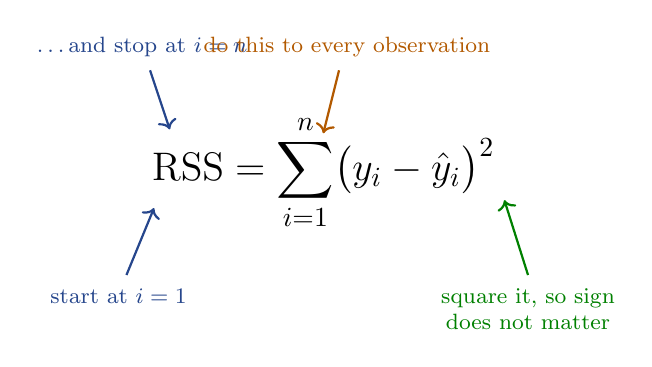
\begin{tikzpicture}[every node/.style={font=\footnotesize}]
      \node[font=\Large] (f) at (0,0) {$\displaystyle \mathrm{RSS} = \sum_{i=1}^{n}\bigl(y_i - \hat y_i\bigr)^2$};
      \draw[->,accent,thick] (-2.5,-1.3) -- (-2.15,-0.45);
      \node[accent,align=center,anchor=north] at (-2.6,-1.35) {start at $i = 1$};
      \draw[->,accent,thick] (-2.2,1.3) -- (-1.95,0.55);
      \node[accent,align=center,anchor=south] at (-2.3,1.35) {\dots and stop at $i = n$};
      \draw[->,orange!70!black,thick] (0.2,1.3) -- (0.0,0.5);
      \node[orange!70!black,align=center,anchor=south] at (0.3,1.35) {do this to every observation};
      \draw[->,green!50!black,thick] (2.6,-1.3) -- (2.3,-0.35);
      \node[green!50!black,align=center,anchor=north] at (2.6,-1.35) {square it, so sign\\does not matter};
    \end{tikzpicture}
  \end{center}
  \begin{takeaway}[How to read any formula]
    Read it as an \emph{instruction}, left to right: ``for each observation,
    take the gap between what happened and what we predicted, square it, and
    add those up''. A formula is a recipe, not a hieroglyph.
  \end{takeaway}
\end{frame}

\begin{frame}{Sums and products}
  \footnotesize
  \begin{block}{The two operators that appear everywhere}
    \[
      \sum_{i=1}^{n} a_i = a_1 + a_2 + \dots + a_n,
      \qquad
      \prod_{i=1}^{n} a_i = a_1 \times a_2 \times \dots \times a_n .
    \]
  \end{block}
  \begin{numexample}[With numbers]
    For $a = (2, 5, 3)$: $\sum_i a_i = 10$ and $\prod_i a_i = 30$.
    In Python: \texttt{a.sum()} and \texttt{a.prod()}.
  \end{numexample}
  \begin{block}{Rules worth knowing}
    \[
      \sum_i (a_i + b_i) = \sum_i a_i + \sum_i b_i,
      \qquad
      \sum_i c\,a_i = c\sum_i a_i,
      \qquad
      \sum_{i=1}^{n} c = nc .
    \]
  \end{block}
  \begin{alertblock}{The one that is \emph{not} a rule}
    $\sum_i a_i b_i \ne \bigl(\sum_i a_i\bigr)\bigl(\sum_i b_i\bigr)$, and
    $\sum_i a_i^2 \ne \bigl(\sum_i a_i\bigr)^2$.
  \end{alertblock}
\end{frame}

\begin{frame}{$\arg\min$, $\arg\max$ and the indicator}
  \footnotesize
  \begin{block}{$\min$ versus $\arg\min$}
    $\min_\theta f(\theta)$ is the smallest \emph{value} of $f$;
    $\arg\min_\theta f(\theta)$ is the \emph{$\theta$ that achieves it}.
    \[
      f(\theta) = (\theta-3)^2 + 5
      \quad\Longrightarrow\quad
      \min_\theta f = 5, \qquad \arg\min_\theta f = 3 .
    \]
    Estimation is always an $\arg\min$ (of a loss) or an $\arg\max$ (of a
    likelihood): we want the \emph{parameter}, not the value of the criterion.
  \end{block}
  \begin{block}{The indicator function}
    \[
      I(\text{condition}) =
      \begin{cases} 1 & \text{if the condition is true},\\ 0 & \text{otherwise.}\end{cases}
    \]
    It turns counting into arithmetic. The classification error rate is
    \[
      \frac{1}{n}\sum_{i=1}^{n} I(y_i \ne \hat y_i)
      \quad\text{---}\quad
      \text{``the fraction of observations we got wrong''.}
    \]
  \end{block}
\end{frame}

\begin{frame}{Sets, subscripts and the notation of a data set}
  \footnotesize
  \begin{block}{Sets}
    $x \in \mathcal{S}$ means ``$x$ belongs to $\mathcal{S}$'';
    $|\mathcal{S}|$ is the number of elements in $\mathcal{S}$.
    In Chapter 8, $R_j$ is the set of observations falling in region $j$ of a
    tree, and $\frac{1}{|R_j|}\sum_{i \in R_j} y_i$ is just ``the mean response
    of the points in that box''.
  \end{block}
  \begin{block}{Subscripts and superscripts}
    \begin{tabular}{@{}ll@{}}
      $x_{ij}$ & observation $i$, variable $j$ (row first, then column) \\
      $x_i$ & the whole $i$-th row (a vector of $p$ numbers) \\
      $\beta_j$ & the coefficient belonging to variable $j$ \\
      $\hat y_i^{(-i)}$ & prediction for $i$ from a model fitted \emph{without} $i$ \\
      $\alpha^{*b}$ & the estimate from bootstrap sample $b$ (a label, not a power) \\
    \end{tabular}
  \end{block}
  \begin{alertblock}{Read the superscript before you square it}
    In Chapter 5, $\hat\alpha^{*b}$ is ``the estimate from resample $b$''.
    A superscript is often an \emph{index}, not an exponent --- context decides.
  \end{alertblock}
\end{frame}

\begin{frame}{Exercise 0b.1 --- Translating notation [Math]}
  \begin{exercise}
    Let $y = (3, 1, 4)$ and $\hat y = (2, 2, 4)$, so $n = 3$.
    \begin{enumerate}
      \item Write $\sum_{i=1}^{3}(y_i - \hat y_i)^2$ in words, then compute it.
      \item Compute $\frac{1}{n}\sum_{i=1}^{n} I(y_i \ne \hat y_i)$ and say what
            it measures.
      \item For $g(\theta) = (\theta - 4)^2 + 7$, give $\min_\theta g$ and
            $\arg\min_\theta g$.
      \item Let $\mathcal{S} = \{i : y_i > 2\}$. List $\mathcal{S}$, give
            $|\mathcal{S}|$, and compute $\frac{1}{|\mathcal{S}|}\sum_{i \in \mathcal{S}} y_i$.
      \item Is $\sum_i (y_i - \hat y_i)^2$ the same as
            $\bigl(\sum_i (y_i - \hat y_i)\bigr)^2$? Check with these numbers.
    \end{enumerate}
  \end{exercise}
\end{frame}

\begin{frame}{Solution --- Exercise 0b.1}
  \begin{solutionbox}
    \textbf{(1)} ``For each of the three observations, subtract the prediction
    from the observation, square the result, and add the three numbers.''
    Differences: $1, -1, 0$; squares $1, 1, 0$; total $\mathbf{2}$.

    \textbf{(2)} The indicator is $1$ for observations $1$ and $2$ (where
    $y_i \neq \hat y_i$) and $0$ for the third, so the average is
    $2/3 \approx 0.67$: \emph{the fraction of predictions that are wrong} ---
    the misclassification rate of Chapters 2 and 4.

    \textbf{(3)} A square is never negative, so $g$ is smallest when
    $(\theta-4)^2 = 0$. Hence $\arg\min_\theta g = \mathbf{4}$ and
    $\min_\theta g = \mathbf{7}$. Note the two answers are different objects:
    one is a parameter, the other a loss value.

    \textbf{(4)} $\mathcal{S} = \{1, 3\}$ (observations with $y_i > 2$), so
    $|\mathcal{S}| = 2$ and the mean over the set is $(3+4)/2 = \mathbf{3.5}$.
    This is exactly the calculation a regression tree does inside one leaf.

    \textbf{(5)} \textbf{No.} Here $\sum_i (y_i - \hat y_i)^2 = 2$ but
    $\bigl(\sum_i (y_i - \hat y_i)\bigr)^2 = (1 - 1 + 0)^2 = 0$. Squaring
    first keeps the errors from cancelling --- which is the whole reason
    least squares squares.
  \end{solutionbox}
\end{frame}


% ============================================================
\section{Logs, exponentials and growth}
% ============================================================

\begin{frame}{The two functions Chapter 4 is written in}
  \begin{center}
    
\includegraphics[width=0.90\textwidth,height=0.46\textheight,keepaspectratio]{ch00b_exp_log.png}
  \end{center}
  \footnotesize
  \begin{block}{The rules, all of them}
    \[
      \log(ab) = \log a + \log b, \quad
      \log(a/b) = \log a - \log b, \quad
      \log(a^{k}) = k\log a,
    \]
    \[
      \log 1 = 0, \quad \log e = 1, \quad
      e^{\log a} = a, \quad \log(e^{x}) = x, \quad
      e^{a+b} = e^{a}e^{b}.
    \]
  \end{block}
  ``$\log$'' in this course always means the \emph{natural} logarithm, base
  $e \approx 2.718$ --- what \texttt{np.log} computes.
\end{frame}

\begin{frame}{Why logs are everywhere in statistics}
  \footnotesize
  \begin{takeaway}[Three jobs a log does]
    \begin{enumerate}
      \item \textbf{Turns multiplying into adding.} A likelihood is a product
            over $n$ observations; its log is a sum, which we can
            differentiate. (Next section.)
      \item \textbf{Turns unbounded ratios into a symmetric scale.} Odds run
            from $0$ to $\infty$; log-odds run from $-\infty$ to $\infty$.
            (Section after that.)
      \item \textbf{Tames skew and turns effects into percentages.} A right tail
            is compressed, and a coefficient on $\log y$ reads as a
            \emph{relative} change.
    \end{enumerate}
  \end{takeaway}
  \begin{numexample}[Numerical underflow --- the practical reason]
    A likelihood multiplies $n$ probabilities. With $n = 1000$ and each
    around $0.5$, the product is $\approx 10^{-301}$, close to the smallest
    number a computer can store; at $n = 2000$ it underflows to zero and every
    model looks equally good. Its log $\approx -693$ is perfectly ordinary.
  \end{numexample}
\end{frame}

\begin{frame}{A log scale can straighten a relationship}
  \begin{center}
    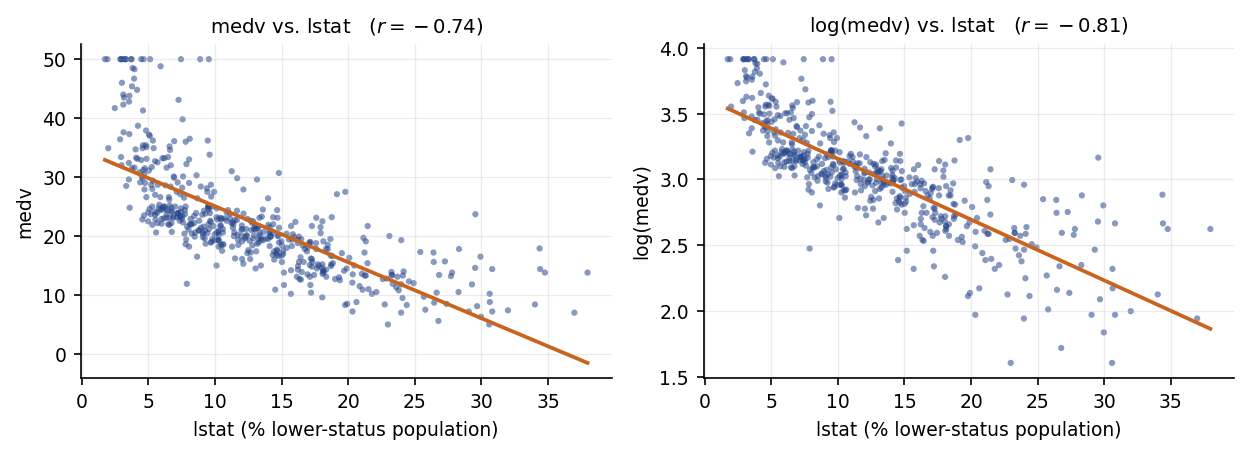
\includegraphics[width=0.90\textwidth,height=0.46\textheight,keepaspectratio]{ch00b_log_scale.png}
  \end{center}
  \footnotesize
  \texttt{Boston}: median house value against the share of lower-status
  population. On the raw scale the cloud curves and $r = -0.74$; after logging
  the response it is close to straight, and $r = -0.81$.
  \begin{takeaway}[How to read a logged coefficient]
    In $\log y = \beta_0 + \beta_1 x$, a one-unit rise in $x$ multiplies $y$ by
    $e^{\beta_1}$. For small $\beta_1$, that is roughly a
    $100\beta_1\%$ change: $\beta_1 = -0.05$ means ``about $5\%$ lower''.
  \end{takeaway}
\end{frame}

\begin{frame}{Exercise 0b.2 --- Logs in practice [Math]}
  \begin{exercise}
    \begin{enumerate}
      \item Simplify $\log(x^3 y) - \log(y)$ and $\log\!\bigl(e^{2x}\bigr)$.
      \item Solve $e^{0.4t} = 5$ for $t$.
      \item A model gives $\log(\text{wage}) = 2.1 + 0.08\,\text{educ}$.
            By what factor does an extra year of education multiply the wage?
            Express it as a percentage.
      \item Prices rise $3\%$ a year. Write the price after $t$ years, take
            logs, and say why the log of the price is a straight line in $t$.
      \item Why can you not take the log of a variable that contains zeros,
            and what do people do instead?
    \end{enumerate}
  \end{exercise}
\end{frame}

\begin{frame}{Solution --- Exercise 0b.2}
  \begin{solutionbox}
    \textbf{(1)} $\log(x^3y) - \log y = \log x^3 + \log y - \log y =
    3\log x$. And $\log(e^{2x}) = 2x$, since $\log$ and $\exp$ undo each
    other.

    \textbf{(2)} Take logs of both sides: $0.4t = \log 5 = 1.609$, so
    $t = 1.609/0.4 = \mathbf{4.02}$.

    \textbf{(3)} An extra year adds $0.08$ to $\log(\text{wage})$, so it
    multiplies the wage by $e^{0.08} = 1.083$: about $\mathbf{+8.3\%}$. Note
    the shortcut ``$0.08 \to 8\%$'' is an approximation that is good for small
    coefficients and poor for large ones ($e^{0.5} = 1.65$, not $1.5$).

    \textbf{(4)} $P_t = P_0(1.03)^t$, so
    $\log P_t = \log P_0 + t\log(1.03) = \log P_0 + 0.0296\,t$. Constant
    \emph{growth rates} are straight lines on a log scale --- which is why
    growth data are always plotted that way.

    \textbf{(5)} $\log 0 = -\infty$ (and logs of negatives are undefined), so a
    single zero destroys the column. Common fixes: model $\log(y + 1)$; use a
    square root instead; or --- best --- use a model built for the data type,
    such as the Poisson regression of Chapter 4 for counts.
  \end{solutionbox}
\end{frame}


% ============================================================
\section{Probability, odds and the logit}
% ============================================================

\begin{frame}{Three ways to say the same thing}
  \footnotesize
  \begin{block}{Definitions}
    \[
      \mathrm{odds} = \frac{p}{1-p},
      \qquad
      \mathrm{logit}(p) = \log\frac{p}{1-p},
      \qquad
      p = \sigma(z) = \frac{1}{1+e^{-z}} .
    \]
  \end{block}
  \begin{center}
  \begin{tabular}{@{}rrrl@{}}
    \toprule
    \textbf{probability} & \textbf{odds} & \textbf{log-odds} & \textbf{said aloud} \\
    \midrule
    $0.10$ & $0.11$ & $-2.20$ & ``$1$ to $9$ against'' \\
    $0.25$ & $0.33$ & $-1.10$ & ``$1$ to $3$ against'' \\
    $0.50$ & $1.00$ & $0.00$  & ``evens'' \\
    $0.75$ & $3.00$ & $+1.10$ & ``$3$ to $1$ on'' \\
    $0.90$ & $9.00$ & $+2.20$ & ``$9$ to $1$ on'' \\
    \bottomrule
  \end{tabular}
  \end{center}
  \begin{takeaway}[Why the log-odds scale]
    Probabilities are squeezed against $0$ and $1$; log-odds run from $-\infty$
    to $+\infty$, symmetrically about zero. Models work on the log-odds scale
    because it has \emph{room}: whatever number a linear predictor produces is
    a legal log-odds.
  \end{takeaway}
\end{frame}

\begin{frame}{The three scales, drawn}
  \begin{center}
    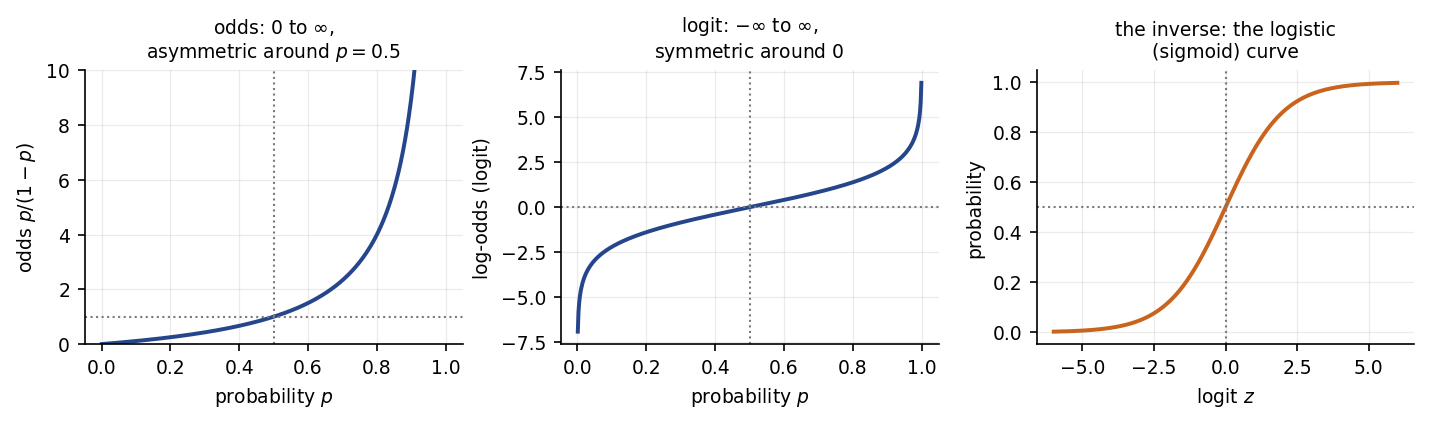
\includegraphics[width=0.99\textwidth,height=0.50\textheight,keepaspectratio]{ch00b_odds_logit.png}
  \end{center}
  \footnotesize
  Left to right: probabilities become odds ($0$ to $\infty$), odds become
  log-odds ($-\infty$ to $\infty$), and the logistic function
  $\sigma(z) = 1/(1+e^{-z})$ carries them back. Because $\sigma$ can never
  leave $(0,1)$, \emph{any} number a linear model produces becomes a legal
  probability.
\end{frame}

\begin{frame}{Why Chapter 4 cannot just fit a straight line}
  \begin{center}
    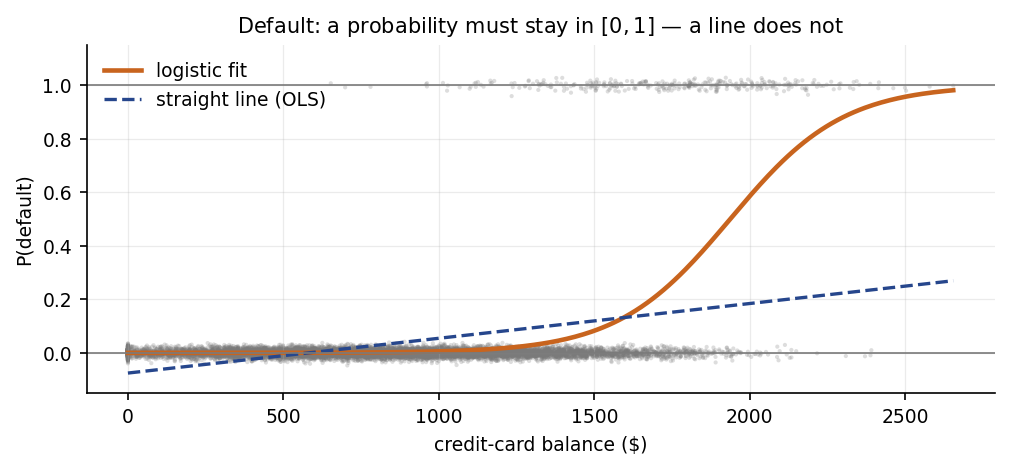
\includegraphics[width=0.82\textwidth,height=0.48\textheight,keepaspectratio]{ch00b_sigmoid_fit.png}
  \end{center}
  \footnotesize
  \texttt{Default} ($n = 10\,000$, $3.3\%$ default). The dashed line is
  ordinary least squares on a $0/1$ response: it predicts \emph{negative}
  probabilities for small balances and would exceed $1$ eventually. The
  logistic curve cannot.
  \begin{takeaway}[The one-line summary of logistic regression]
    Model the \emph{log-odds} as linear:
    $\log\frac{p(x)}{1-p(x)} = \beta_0 + \beta_1 x$, then convert back with
    $\sigma$. That is the whole idea; Chapter 4 fills in the details.
  \end{takeaway}
\end{frame}

\begin{frame}{Exercise 0b.3 --- Odds and odds ratios [Math]}
  \begin{exercise}
    In a promotion study, $45\%$ of customers who received a voucher bought
    something, against $25\%$ of those who did not.
    \begin{enumerate}
      \item Compute the odds of buying in each group.
      \item Compute the \textbf{odds ratio} (voucher vs.\ no voucher) and state
            in words what it says.
      \item Compute the log-odds in each group, and check that their
            difference equals the log of the odds ratio.
      \item A logistic model reports a coefficient of $0.90$ for the voucher
            dummy. Convert it to an odds ratio.
      \item If the log-odds of an outcome are $-1.4$, what is the probability?
    \end{enumerate}
  \end{exercise}
\end{frame}

\begin{frame}{Solution --- Exercise 0b.3}
  \begin{solutionbox}
    \textbf{(1)} Voucher: $0.45/0.55 = \mathbf{0.818}$. No voucher:
    $0.25/0.75 = \mathbf{0.333}$.

    \textbf{(2)} Odds ratio $= 0.818/0.333 = \mathbf{2.45}$: the \emph{odds} of
    buying are about two and a half times higher with a voucher. Note this is
    not ``2.45 times as likely'' --- the ratio of \emph{probabilities} is only
    $0.45/0.25 = 1.8$. Odds ratios and risk ratios are different numbers, and
    confusing them overstates effects.

    \textbf{(3)} $\log 0.818 = -0.201$ and $\log 0.333 = -1.099$; the
    difference is $0.898 = \log(2.45)$ \checkmark. \emph{Differences on the
    log-odds scale are ratios on the odds scale} --- which is exactly what a
    logistic coefficient is.

    \textbf{(4)} $e^{0.90} = \mathbf{2.46}$ --- the same odds ratio, as it must
    be: the coefficient of a dummy \emph{is} the log odds ratio.

    \textbf{(5)} $p = \sigma(-1.4) = 1/(1 + e^{1.4}) = 1/(1+4.055) =
    \mathbf{0.198}$, about $20\%$.
  \end{solutionbox}
\end{frame}


% ============================================================
\section{Likelihood and maximum likelihood}
% ============================================================

\begin{frame}{The idea in one sentence}
  \begin{takeaway}[Maximum likelihood]
    Among all parameter values, choose the one that makes the data you
    actually observed \emph{most probable}.
  \end{takeaway}
  \footnotesize
  \begin{block}{The likelihood function}
    For independent observations $y_1,\dots,y_n$ with parameter $\theta$,
    \[
      L(\theta) = \prod_{i=1}^{n} P(y_i \mid \theta),
      \qquad
      \ell(\theta) = \log L(\theta) = \sum_{i=1}^{n} \log P(y_i \mid \theta) .
    \]
  \end{block}
  \begin{readme}[Read the direction of the conditioning]
    $P(y_i \mid \theta)$ is a probability \emph{of the data given a parameter}.
    As a function of $\theta$ with the data \emph{fixed}, we call it a
    likelihood --- and it is \textbf{not} a probability distribution over
    $\theta$. That is the commonest misunderstanding here.
  \end{readme}
\end{frame}

\begin{frame}{A coin, worked end to end}
  \begin{center}
    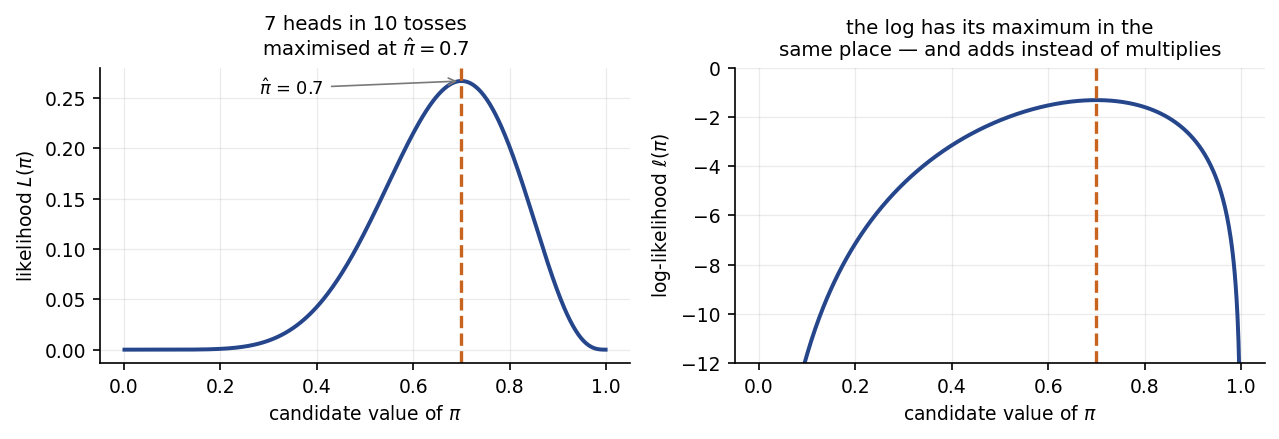
\includegraphics[width=0.88\textwidth,height=0.44\textheight,keepaspectratio]{ch00b_likelihood_coin.png}
  \end{center}
  \footnotesize
  Seven heads in ten tosses. The likelihood
  $L(\pi) = \binom{10}{7}\pi^{7}(1-\pi)^{3}$ peaks at $\hat\pi = 0.7$; the
  log-likelihood peaks in the same place, because $\log$ is increasing.
  \begin{takeaway}[Why we always maximise the log]
    Same answer, easier algebra (sums, not products), and no numerical
    underflow. Every ``log-likelihood'' in Chapters 4, 6 and 10 is this.
  \end{takeaway}
\end{frame}





\begin{frame}{Exercise 0b.4 --- What a likelihood is and is not [Concept]}
  \begin{exercise}
    Decide whether each statement is correct, and correct the ones that are
    not.
    \begin{enumerate}
      \item ``The likelihood that $\pi = 0.7$ is $0.27$, so there is a 27\%
            chance the true value is $0.7$.''
      \item ``The maximum-likelihood estimate is the most probable value of
            the parameter.''
      \item ``Adding an observation always lowers the likelihood.''
      \item ``Maximising the likelihood and maximising the log-likelihood can
            give different answers.''
      \item ``A model with a higher log-likelihood always predicts new data
            better.''
    \end{enumerate}
  \end{exercise}
\end{frame}

\begin{frame}{Solution --- Exercise 0b.4}
  \begin{solutionbox}
    \textbf{(1) Wrong.} A likelihood is a probability of the \emph{data},
    computed \emph{given} a parameter value --- not a probability of the
    parameter. Likelihoods need not sum or integrate to $1$ over $\pi$, so
    ``27\% chance'' is meaningless here. (Turning it into a statement about
    $\pi$ requires a prior and Bayes' theorem.)

    \textbf{(2) Wrong, in the same way.} It is the value \emph{under which the
    observed data are most probable}. The distinction matters exactly when
    someone asks ``how sure are you?'' --- that question is answered by a
    standard error or an interval, not by the likelihood's height.

    \textbf{(3) Correct for discrete data.} Each extra observation multiplies
    in another probability $\le 1$, so $L$ shrinks; for a continuous response
    the factors are densities and can exceed $1$. Only \emph{comparisons at
    the same data set} are meaningful ---
    which is why you can never compare log-likelihoods across samples of
    different size.

    \textbf{(4) Wrong.} $\log$ is strictly increasing, so it preserves the
    location of the maximum. The maximiser is identical; only the value
    differs.

    \textbf{(5) Wrong.} Likelihood is measured on the \emph{training} data, and
    a more flexible model can always be made to fit it better --- overfitting.
    That is precisely why Chapter 6 penalises the log-likelihood (AIC, BIC) and
    Chapter 5 measures performance on held-out data instead.
  \end{solutionbox}
\end{frame}


% ============================================================
\section{The Python you will actually write}
% ============================================================

\begin{frame}[fragile]{Functions and loops --- used in all fifteen labs}
\begin{lstlisting}
def rmse(y, y_hat):                     # define once, reuse everywhere
    """Root mean squared error."""
    return np.sqrt(np.mean((y - y_hat) ** 2))

scores = []                             # accumulate results in a list
for degree in range(1, 6):              # range(1, 6) -> 1, 2, 3, 4, 5
    fit = np.polyfit(x_train, y_train, degree)
    scores.append(rmse(y_test, np.polyval(fit, x_test)))

best = int(np.argmin(scores)) + 1       # argmin gives the POSITION
print(f"best degree: {best}  (RMSE {min(scores):.3f})")
\end{lstlisting}
  \begin{takeaway}[The pattern behind every tuning experiment]
    Define a scoring function; loop over candidate settings; store each score;
    take the \texttt{argmin}. Chapters 5--8 change what happens inside the
    loop, never the shape of it.
  \end{takeaway}
\end{frame}

\begin{frame}[fragile]{Four idioms worth ten minutes each}
\begin{lstlisting}
squares = [d ** 2 for d in range(5)]          # list comprehension
mask = df["balance"] > 1000                   # a boolean Series...
df.loc[mask, "income"].mean()                 # ...used to select rows

for name, group in df.groupby("education"):   # iterate over groups
    print(name, group["wage"].median())

for ax, col in zip(axes.ravel(), columns):    # zip pairs things up
    ax.hist(df[col])
\end{lstlisting}
  \begin{alertblock}{Two things that will bite you}
    \begin{enumerate}
      \item \textbf{Indexing starts at 0}, and \texttt{range(1, 6)} \emph{excludes}
            6. Off-by-one errors are the most common lab bug.
      \item \textbf{Chained assignment}: \texttt{df[df.x > 1]["y"] = 0} silently
            does nothing. Use \texttt{df.loc[df.x > 1, "y"] = 0}.
    \end{enumerate}
  \end{alertblock}
\end{frame}

\begin{frame}[fragile]{Randomness, seeds and reproducibility}
\begin{lstlisting}
rng = np.random.default_rng(2024)        # ONE generator, seeded once
sample = rng.choice(data, size=100)

from sklearn.model_selection import train_test_split
X_tr, X_te, y_tr, y_te = train_test_split(X, y, test_size=0.3,
                                          random_state=42)
\end{lstlisting}
  \begin{center}
    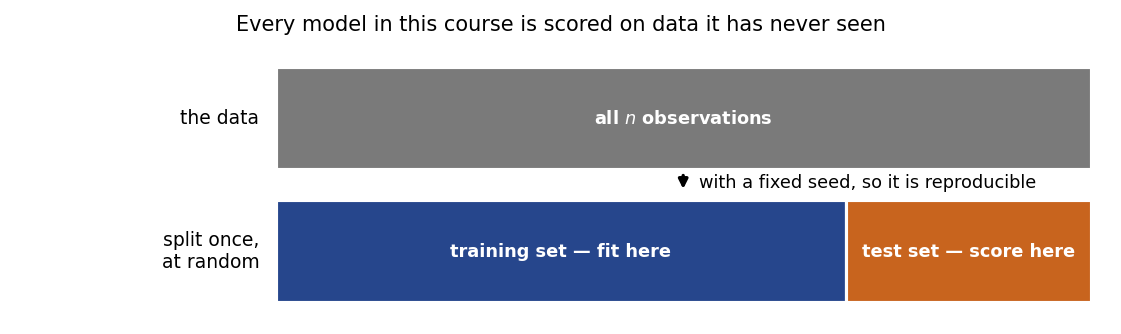
\includegraphics[width=0.90\textwidth,height=0.31\textheight,keepaspectratio]{ch00b_split.png}
  \end{center}
  \scriptsize
  A ``random'' generator is a deterministic recipe and the seed is where it
  starts, so the same seed replays the same draws --- which is why your numbers
  match the slides. Change the seed and the third decimal moves: not a bug, but
  sampling variability, which Chapter 5 is about measuring.
\end{frame}

\begin{frame}[fragile]{The scikit-learn contract: fit, predict, score}
\begin{lstlisting}
from sklearn.linear_model import LinearRegression
from sklearn.metrics import mean_squared_error

model = LinearRegression()               # 1. choose a model
model.fit(X_train, y_train)              # 2. learn from TRAINING data only
pred  = model.predict(X_test)            # 3. predict on unseen data
mean_squared_error(y_test, pred)         # 4. score honestly
model.coef_, model.intercept_            # fitted values carry a trailing _
\end{lstlisting}
  \begin{takeaway}[Learn it once and you know every model in the course]
    Trees, forests, boosting, SVMs and neural nets use the same three methods:
    swapping \texttt{LinearRegression()} for
    \texttt{RandomForestRegressor()} changes one line.
  \end{takeaway}
  \begin{alertblock}{The cardinal sin}
    Never call \texttt{fit} on the test set --- not for the model, and not for
    a scaler either (Chapter 5).
  \end{alertblock}
\end{frame}

\begin{frame}[fragile]{Exercise 0b.6 --- Reading and fixing code [Python]}
  \begin{exercise}
    \scriptsize
    A student writes the following to compare polynomial degrees:
\begin{lstlisting}
scores = []
for degree in range(1, 5):
    fit = np.polyfit(x, y, degree)              # (a)
    scores.append(rmse(y, np.polyval(fit, x)))  # (b)
best = np.argmin(scores)                        # (c)
print("best degree:", best)
\end{lstlisting}
    \begin{enumerate}
      \item Which degrees are actually tried?
      \item Line (c) prints \texttt{3} for the best degree. Why is that
            answer wrong, and what is the correct degree?
      \item Lines (a) and (b) use the same data. What will \texttt{scores}
            look like as the degree rises, and why does that make the
            comparison meaningless?
      \item Rewrite the loop so the comparison is honest. Name the one
            function you need.
      \item Why should the code set a seed?
    \end{enumerate}
  \end{exercise}
\end{frame}

\begin{frame}[fragile]{Solution --- Exercise 0b.6}
  \begin{solutionbox}
    \scriptsize
    \textbf{(1)} \texttt{range(1, 5)} yields $1, 2, 3, 4$ --- the upper limit is
    \emph{excluded}. Degree 5 is never tried.

    \textbf{(2)} \texttt{np.argmin} returns a \emph{position}, and positions
    start at $0$. Position $3$ is the fourth entry, i.e.\ degree
    $\mathbf{4}$. The fix is \texttt{best = np.argmin(scores) + 1}, or better,
    store the degrees alongside the scores.

    \textbf{(3)} The model is scored on the same data it was fitted to, so the
    RMSE can only fall as the degree rises --- a high enough polynomial passes
    through every point and scores $0$. The loop therefore always ``discovers''
    the most complex model. This is overfitting, the central problem of
    Chapter 2.

    \textbf{(4)} Split first, fit on training data, score on test data:
\begin{lstlisting}
X_tr, X_te, y_tr, y_te = train_test_split(x, y, test_size=.3, random_state=1)
for degree in range(1, 6):
    fit = np.polyfit(X_tr, y_tr, degree)
    scores.append(rmse(y_te, np.polyval(fit, X_te)))
\end{lstlisting}
    The function is \texttt{sklearn.model\_selection.train\_test\_split}
    (Chapter 5 replaces it with cross-validation).

    \textbf{(5)} Without a seed the split differs on every run, so the ``best''
    degree changes between runs and neither you nor a reader can reproduce the
    number. A seed makes the result checkable --- it does not make it correct.
  \end{solutionbox}
\end{frame}

\begin{frame}{Extended Exercise 0b.2 --- A complete small experiment [Python]}
  \begin{longexercise}
    You are given \texttt{Auto} and want to know how well \texttt{horsepower}
    predicts \texttt{mpg}, and whether a curve beats a line.
    \begin{enumerate}
      \item Write, in words or code, the six steps of the experiment from
            loading the data to reporting a number.
      \item Which step must come \emph{before} any model is fitted, and why?
      \item On one $70/30$ split you get test RMSEs
            $4.96,\ 4.52,\ 4.54,\ 4.55,\ 4.44$ for degrees $1$ to $5$. Which
            degree do you choose, and which part of that sequence is real?
      \item Rerunning with $30$ different seeds, degree $5$ wins $21$ times,
            degree $2$ six times and degree $3$ three times. What does that
            tell you about your answer to (3), and what would you do about it?
      \item Your colleague standardised \texttt{horsepower} using the mean and
            SD of the \emph{whole} data set before splitting. Explain the
            problem in one sentence.
    \end{enumerate}
  \end{longexercise}
\end{frame}

\begin{frame}{Solution --- Extended Exercise 0b.2}
  \begin{solutionbox}
    \scriptsize
    \textbf{(1) The six steps.} Load; \emph{look} at it (scatter, and check
    for missing values --- \texttt{Auto} stores them as \texttt{'?'}); split
    with a seed; fit each candidate on the training set; score each on the
    test set; report the chosen model \emph{with} its test error.

    \textbf{(2) Looking, and splitting.} Plot before modelling --- the
    curvature is obvious and tells you a polynomial is worth trying. And the
    split must precede every fitting decision, so that nothing you learn from
    the test set can influence the model.

    \textbf{(3) Only the first step is real.} The drop from $4.96$ to $4.52$
    is large and reflects genuine curvature: a line is the wrong shape. After
    that the numbers differ by less than $0.12$, which is the size of ordinary
    split-to-split noise. Degree $5$ is nominally lowest, but nothing
    meaningful separates it from degree $2$ --- so choose \textbf{degree 2},
    the simplest model that is not beaten.

    \textbf{(4) The winner is unstable, so do not trust it.} A single split is
    a high-variance estimate, and the seed sweep proves it: three different
    ``best'' degrees appear. Use $k$-fold cross-validation (Chapter 5), which
    averages over splits.
    Doing that here ($5$-fold, repeated $10\times$) gives RMSEs of
    $4.91,\ 4.36,\ 4.37,\ 4.38,\ 4.34$ with a repeat-to-repeat spread of about
    $\pm0.04$: degree $1$ is clearly worse, and \emph{degrees 2 to 5 are
    statistically indistinguishable}. The defensible sentence is ``a quadratic
    is a real improvement on a line; beyond that this data set cannot tell''.

    \textbf{(5) Leakage.} The scaler learned the mean and SD from data that
    includes the test set, so information from the test set has entered the
    training pipeline and the test error is no longer an honest estimate of
    performance on new data (fit the scaler on the training set alone).
  \end{solutionbox}
\end{frame}


% ============================================================
\section{Summary}
% ============================================================

\begin{frame}{The session in one slide}
  \footnotesize
  \begin{itemize}
    \item \textbf{Notation} is instructions: $\sum$ add, $\prod$ multiply,
          $\arg\min$ ``the value that minimises'', $I(\cdot)$ a $0/1$ switch,
          $|\mathcal{S}|$ a count. Read formulas aloud.
    \item \textbf{Logs} turn products into sums, ratios into differences and
          skew into symmetry; $e^{\beta}$ converts a logged coefficient back
          into a multiplicative effect.
    \item \textbf{Odds} $= p/(1-p)$; \textbf{logit} $= \log$ odds, on
          $(-\infty,\infty)$; $\sigma$ brings it back to $(0,1)$. Logistic
          regression is a linear model \emph{on the logit scale}.
    \item \textbf{Likelihood} is the probability of the observed data as a
          function of the parameter; maximise its log. Under normal errors this
          is least squares; under Bernoulli it gives $k/n$ and, with
          predictors, logistic regression.
    \item \textbf{Counting} explains Chapter 6: $2^p$ subsets is hopeless,
          $p^2/2$ is not.
    \item \textbf{Python}: a function, a loop, a seed, and
          \texttt{fit}/\texttt{predict} on a split --- that is every lab.
  \end{itemize}
\end{frame}

\begin{frame}{Key formulas at a glance}
  \footnotesize
  \begin{block}{Notation}
    \[
      \sum_{i=1}^{n} a_i, \quad \prod_{i=1}^{n} a_i, \quad
      \arg\min_\theta f(\theta), \quad
      \frac{1}{n}\sum_{i=1}^n I(y_i \ne \hat y_i) .
    \]
  \end{block}
  \begin{block}{Logs, odds and the logistic function}
    \[
      \log(ab) = \log a + \log b, \qquad \log(a^k) = k \log a,
    \]
    \[
      \mathrm{odds} = \frac{p}{1-p}, \qquad
      \mathrm{logit}(p) = \log\frac{p}{1-p}, \qquad
      \sigma(z) = \frac{1}{1+e^{-z}} .
    \]
  \end{block}
  \begin{block}{Likelihood and counting}
    \[
      \ell(\theta) = \sum_{i=1}^{n}\log P(y_i \mid \theta),
      \qquad
      \hat\theta = \arg\max_\theta \ell(\theta),
      \qquad
      \binom{p}{k}, \quad \sum_{k=0}^p \binom{p}{k} = 2^p .
    \]
  \end{block}
\end{frame}

\begin{frame}{Vocabulary check}
  \scriptsize
  \begin{center}
  \begin{tabular}{@{}ll@{}}
    \toprule
    \textbf{Term} & \textbf{One-line meaning} \\
    \midrule
    Summation / product notation & compact instructions to add or multiply \\
    Indicator function & a $0/1$ switch that turns counting into arithmetic \\
    $\arg\min$ / $\arg\max$ & the input that minimises / maximises, not the value \\
    Natural logarithm & the inverse of $e^x$; \texttt{np.log} \\
    Odds & $p/(1-p)$: how much more likely than not \\
    Odds ratio & ratio of two odds --- what a logistic coefficient exponentiates to \\
    Logit & log-odds; the scale on which classification is linear \\
    Logistic / sigmoid & $\sigma(z) = 1/(1+e^{-z})$; maps any number into $(0,1)$ \\
    Likelihood & probability of the observed data, as a function of the parameter \\
    Log-likelihood & its log: sums instead of products, no underflow \\
    Maximum likelihood & the parameter that makes the observed data most probable \\
    Cross-entropy & $-\ell$ for a classifier; the loss of Chapter 10 \\
    Binomial coefficient & $\binom{p}{k}$: the number of subsets of size $k$ \\
    Data leakage & letting test information reach the training pipeline \\
    Seed & fixes the random draw so results are reproducible \\
    \bottomrule
  \end{tabular}
  \end{center}
\end{frame}

\begin{frame}{Where each topic reappears in the course}
  \footnotesize
  \begin{center}
  \begin{tabular}{@{}ll@{}}
    \toprule
    \textbf{Topic from this session} & \textbf{Comes back in} \\
    \midrule
    $\sum$, $\prod$, $\arg\min$, $I(\cdot)$ & every chapter; RSS and error rates from Ch.\ 2 \\
    Sets and $|\mathcal{S}|$ & Ch.\ 8 (tree regions), Ch.\ 12 (clusters) \\
    Logs and exponentials & Ch.\ 3 (logged responses), Ch.\ 4, Ch.\ 10 \\
    Odds, logits, the sigmoid & Ch.\ 4 (logistic regression), Ch.\ 10 (activations) \\
    Likelihood and log-likelihood & Ch.\ 4 (fitting), Ch.\ 6 (AIC, BIC) \\
    Maximum likelihood & Ch.\ 4, Ch.\ 6, Ch.\ 10 (cross-entropy) \\
    $2^p$ and counting & Ch.\ 6 (subset selection) \\
    Loops, functions, \texttt{argmin} & every lab; tuning loops in Ch.\ 5--8 \\
    Seeds and splits & Ch.\ 2 onwards; formalised in Ch.\ 5 \\
    \texttt{fit} / \texttt{predict} & every model in the course \\
    Leakage & Ch.\ 5 (the rule), Ch.\ 6 (scaling inside CV) \\
    \bottomrule
  \end{tabular}
  \end{center}
\end{frame}

\begin{frame}{Common pitfalls to leave behind}
  \begin{alertblock}{Don't}
    \begin{enumerate}
      \item Confuse $\min$ with $\arg\min$, or a value with an index.
      \item Read $\hat\alpha^{*b}$ as a power --- superscripts are often labels.
      \item Write $\sum_i a_i^2 = (\sum_i a_i)^2$. It is false, and it is the
            reason squared errors work.
      \item Report an odds ratio as if it were a ratio of probabilities.
      \item Say ``the likelihood that the parameter is $0.3$''. Likelihood is
            about the \emph{data}, given the parameter.
      \item Take logs of a variable containing zeros without saying what you did.
      \item Score a model on the data it was fitted to.
      \item Forget the seed --- or change it until the answer looks better.
    \end{enumerate}
  \end{alertblock}
\end{frame}

\begin{frame}{Self-check questions}
  \begin{enumerate}
    \item Read $\frac{1}{n}\sum_{i=1}^{n} I(y_i \ne \hat y_i)$ aloud, in words.
    \item What is the difference between $\min_\theta f$ and $\arg\min_\theta f$?
    \item Simplify $\log(a^2 b) - 2\log a$.
    \item A logistic coefficient is $-0.7$. What happens to the odds?
    \item Convert log-odds $+1.6$ into a probability.
    \item Why is a log-likelihood a sum when a likelihood is a product?
    \item Under what assumption is least squares equivalent to maximum
          likelihood?
    \item How many models does best-subset selection fit with $p = 20$?
    \item What does \texttt{np.argmin} return --- and what does it not return?
    \item Name two things that must never be fitted on the test set.
  \end{enumerate}
\end{frame}

\begin{frame}{Five things to remember}
  \begin{enumerate}
    \item \textbf{A formula is a recipe.} Read it aloud as an instruction and
          it stops being intimidating.
    \item \textbf{Logs convert.} Products to sums, ratios to differences,
          growth to straight lines, coefficients to percentages.
    \item \textbf{Classification lives on the logit scale}, because
          probabilities do not have room to be linear.
    \item \textbf{Maximum likelihood is one principle} behind least squares,
          logistic regression, AIC/BIC and cross-entropy.
    \item \textbf{Fit on training data, score on test data, seed everything.}
          Every lab, every chapter, no exceptions.
  \end{enumerate}
\end{frame}

\begin{frame}{What's next}
  Lecture 1 --- \emph{Chapter 1: Introduction} and the start of
  \emph{Chapter 2: Statistical Learning}.
  \begin{itemize}
    \item $Y = f(X) + \varepsilon$: what statistical learning is trying to do.
    \item Prediction versus inference; supervised versus unsupervised.
    \item The course data sets and the notation that goes with them.
  \end{itemize}
  \begin{labnote}[Companion notebook]
    \texttt{Lab\_Notebooks/chapter\_00b\_lab.ipynb} runs everything in this
    deck: the logit conversions, a likelihood maximised by hand and by
    \texttt{scipy}, the $2^p$ count, and a complete
    split/fit/score experiment on \texttt{Auto}.
  \end{labnote}
\end{frame}


% ============================================================
\appendix
\AtBeginSection[]{}
\section{Appendix: optional and advanced material}
% ============================================================

\begin{frame}{Appendix --- what is in here, and why}
  \small
  Nothing in the appendix is needed to follow the chapter: each slide is a
  formal derivation, a longer worked exercise, or a side topic. Read it when
  you want the full story, or when a later chapter sends you back here.
  \begin{block}{Contents of the appendix}
    \begin{itemize}
      \item \textbf{Least squares as maximum likelihood} --- the derivation that connects Chapter 3 to Chapter 4, plus Extended Exercise 0b.1 (deriving an estimator from scratch). The two methods are usable without it.
      \item \textbf{Counting and computational cost} --- how the $2^p$ models of Chapter 6 explode, and why ``just try everything'' fails (with Exercise 0b.5). Chapter 6 re-states the conclusion where it is needed.
    \end{itemize}
  \end{block}
\end{frame}

\begin{frame}{Least squares is maximum likelihood in disguise}
  \begin{center}
    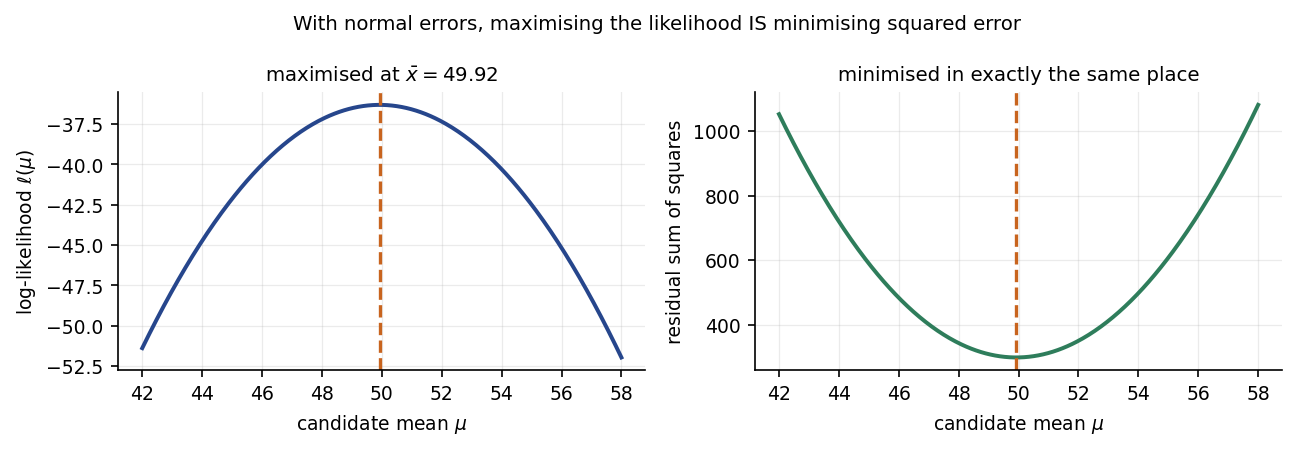
\includegraphics[width=0.88\textwidth,height=0.36\textheight,keepaspectratio]{ch00b_likelihood_normal.png}
  \end{center}
  \footnotesize
  With normal errors $P(y_i \mid \mu) = \frac{1}{\sigma\sqrt{2\pi}}
  \exp\bigl(-\tfrac{(y_i-\mu)^2}{2\sigma^2}\bigr)$, and the log strips the
  exponential down to its exponent:
  $\log P(y_i \mid \mu) = -\frac{(y_i-\mu)^2}{2\sigma^2} + \text{const}$, so
  \[
    \ell(\mu) = -\frac{1}{2\sigma^2}\sum_i (y_i - \mu)^2 + \text{const}
    \quad\Longrightarrow\quad
    \arg\max_\mu \ell(\mu) = \arg\min_\mu \sum_i (y_i-\mu)^2 .
  \]
  \begin{takeaway}[One principle under two names]
    Maximising the likelihood \emph{is} minimising squared error whenever the
    errors are normal. Chapter 4 keeps the principle and drops the normal
    assumption --- that is all logistic regression does.
  \end{takeaway}
\end{frame}

\begin{frame}{Extended Exercise 0b.1 --- Deriving an estimator [Math]}
  \begin{longexercise}
    In a sample of $n$ customers, $k$ default. Model each customer as an
    independent Bernoulli trial with unknown default probability $\pi$.
    \begin{enumerate}
      \item Write the likelihood $L(\pi)$ as a product, then simplify it to a
            single expression in $\pi$, $k$ and $n$.
      \item Take logs to get $\ell(\pi)$.
      \item Differentiate $\ell$ with respect to $\pi$, set the derivative to
            zero, and solve. What is $\hat\pi_{\mathrm{MLE}}$?
      \item Evaluate it for the \texttt{Default} data: $n = 10\,000$ with
            $333$ defaults.
      \item Explain why maximising $\ell$ gives the same answer as maximising
            $L$, and why we bother with the log at all.
      \item Chapter 4 replaces the single $\pi$ by
            $\pi(x_i) = \sigma(\beta_0 + \beta_1 x_i)$. Write the resulting
            log-likelihood, and say why it can no longer be solved by hand.
    \end{enumerate}
  \end{longexercise}
\end{frame}

\begin{frame}{Solution --- Extended Exercise 0b.1 (1/2)}
  \begin{solutionbox}
    \textbf{(1) The likelihood.} Each defaulting customer contributes $\pi$ and
    each non-defaulting one $1-\pi$; independence lets us multiply:
    \[
      L(\pi) = \prod_{i=1}^{n} \pi^{y_i}(1-\pi)^{1-y_i}
             = \pi^{k}(1-\pi)^{\,n-k},
      \qquad k = \sum_i y_i .
    \]
    The exponent trick is worth noticing: $\pi^{y_i}(1-\pi)^{1-y_i}$ equals
    $\pi$ when $y_i = 1$ and $1-\pi$ when $y_i = 0$.

    \textbf{(2) The log-likelihood.}
    \[
      \ell(\pi) = k\log \pi + (n-k)\log(1-\pi).
    \]
    The product has become a sum --- the only reason this is doable by hand.

    \textbf{(3) Maximise.}
    \[
      \frac{d\ell}{d\pi} = \frac{k}{\pi} - \frac{n-k}{1-\pi} = 0
      \;\Longrightarrow\;
      k(1-\pi) = (n-k)\pi
      \;\Longrightarrow\;
      \hat\pi_{\mathrm{MLE}} = \frac{k}{n}.
    \]
    The sample proportion --- exactly what anyone would have guessed. That is
    the point: maximum likelihood \emph{derives} the obvious estimator, and
    keeps working when the answer is no longer obvious.
  \end{solutionbox}
\end{frame}

\begin{frame}{Solution --- Extended Exercise 0b.1 (2/2)}
  \begin{solutionbox}
    \textbf{(4) The numbers.} $\hat\pi = 333/10\,000 = \mathbf{0.0333}$, the
    $3.3\%$ default rate quoted in Chapter 4.

    \textbf{(5) Why the log is safe --- and necessary.} $\log$ is strictly
    increasing, so it preserves the location of the maximum: if
    $L(a) > L(b)$ then $\ell(a) > \ell(b)$. We use it because it converts the
    product into a sum (so the derivative is a sum of simple terms) and because
    the product itself underflows to zero on a computer for even moderate $n$.

    \textbf{(6) The regression version.} With
    $\pi_i = \sigma(\beta_0 + \beta_1 x_i)$,
    \[
      \ell(\beta_0,\beta_1) = \sum_{i=1}^{n}
        \Bigl[\,y_i \log \pi_i + (1-y_i)\log(1-\pi_i)\Bigr].
    \]
    Setting the derivatives to zero now gives equations in which
    $\beta$ appears \emph{inside} $\sigma$, so they cannot be rearranged into
    a closed form as the normal equations were. Software maximises $\ell$
    numerically --- by walking uphill, exactly the gradient method of
    Part (a). Note also that $-\ell$ is the ``binary cross-entropy'' loss of
    Chapter 10: the same quantity under a different name.
  \end{solutionbox}
\end{frame}

\begin{frame}{How many models are there?}
  \footnotesize
  \begin{block}{Counting rules}
    \[
      k! = k(k-1)\cdots 1,
      \qquad
      \binom{p}{k} = \frac{p!}{k!\,(p-k)!},
      \qquad
      \sum_{k=0}^{p}\binom{p}{k} = 2^{p}.
    \]
    $\binom{p}{k}$ counts the subsets of size $k$; summing over all $k$ counts
    \emph{every} subset --- each variable is either in or out, hence $2^p$.
  \end{block}
  \begin{numexample}[With numbers]
    With $p = 4$ predictors there are $\binom{4}{2} = 6$ two-variable models
    and $2^4 = 16$ models in total (including the empty one). With
    $p = 10$: $1\,024$. With $p = 40$: over $10^{12}$.
  \end{numexample}
  \begin{takeaway}[Where you meet this]
    Chapter 6 asks which subset of predictors to keep. The count above is why
    ``try them all'' stops being possible around $p = 30$, and why stepwise
    selection and regularisation exist at all.
  \end{takeaway}
\end{frame}

\begin{frame}{The cost of ``just try everything''}
  \begin{center}
    
\includegraphics[width=0.95\textwidth,height=0.58\textheight,keepaspectratio]{ch00b_subset_growth.png}
  \end{center}
  \footnotesize
  Forward stepwise selection fits about $p^2/2$ models instead of $2^p$: for
  $p = 40$, roughly $800$ instead of $10^{12}$. At $0.01$ s per fit that is
  eight seconds against about $350$ years --- with no guarantee of finding the
  same answer, which is the trade-off Chapter 6 discusses.
\end{frame}

\begin{frame}{Exercise 0b.5 --- Counting [Math]}
  \begin{exercise}
    A data set has $p = 6$ candidate predictors.
    \begin{enumerate}
      \item How many models contain exactly two predictors?
      \item How many models are there in total?
      \item Best-subset selection fits all of them; forward stepwise fits
            $1 + p(p+1)/2$. Compute both counts.
      \item Each fit takes $0.01$ seconds. How long does each strategy take
            for $p = 6$, and for $p = 30$?
      \item Testing every model against the data and keeping the best
            $R^2$ has a statistical cost as well as a computational one. What
            is it? (One sentence; Chapter 13 gives it a name.)
    \end{enumerate}
  \end{exercise}
\end{frame}

\begin{frame}{Solution --- Exercise 0b.5}
  \begin{solutionbox}
    \textbf{(1)} $\binom{6}{2} = \frac{6 \cdot 5}{2} = \mathbf{15}$.

    \textbf{(2)} $2^6 = \mathbf{64}$ (the empty model included).

    \textbf{(3)} Best subset: $64$ fits. Forward stepwise:
    $1 + 6(7)/2 = \mathbf{22}$ fits. For $p = 30$ the same formulas give
    $2^{30} \approx 1.07\times10^{9}$ against $466$.

    \textbf{(4)} At $0.01$ s per fit and $p = 6$: $0.64$ s versus $0.22$ s ---
    no practical difference. At $p = 30$: $1.07\times10^{7}$ seconds
    $\approx \mathbf{124\ \text{days}}$ versus $4.7$ seconds. This is why
    Chapter 6 does not simply recommend best-subset selection.

    \textbf{(5)} Picking the winner from a huge number of models is
    \emph{selection on noise}: with enough candidates, some model fits the
    sample well by luck, so its $R^2$ is optimistic and it may not generalise.
    That is \textbf{multiple testing} (Chapter 13), and it is also why model
    choice must be judged on held-out data (Chapter 5).
  \end{solutionbox}
\end{frame}

\end{document}
